% ======================================================================
%  RAPPORT DE STAGE OPÉRATEUR
%  Lina Assabane — École Centrale Casablanca
%  Reminex (Groupe Managem) — Direction Ingénierie / Process Engineering
%
%  Compilation (Overleaf : pdfLaTeX + Biber) :
%     pdflatex main → biber main → pdflatex main → pdflatex main
% ======================================================================
\documentclass[12pt,a4paper,oneside]{report}

% ======================================================================
%  PRÉAMBULE — Rapport de stage opérateur
%  (packages, mise en page, couleurs, commandes personnalisées)
% ======================================================================

% ---- Langue et encodage ---------------------------------------------
\usepackage[T1]{fontenc}
\usepackage[utf8]{inputenc}
\usepackage[french]{babel}      % typographie française
\usepackage{lmodern}
\usepackage{csquotes}

% ---- Mise en page ---------------------------------------------------
\usepackage[a4paper,margin=2.5cm,headheight=15pt]{geometry}
\usepackage{setspace}
\onehalfspacing                 % interligne 1.5 (consigne ECC)
\usepackage{microtype}

% ---- Graphisme ------------------------------------------------------
\usepackage{graphicx}
\usepackage{xcolor}
\usepackage{caption}            % pour \captionof hors flottant
\usepackage{tikz}
\usetikzlibrary{shapes.geometric,arrows.meta,positioning,calc,chains,fit,backgrounds}
\usepackage{pgfplots}
\pgfplotsset{compat=1.18}
\usepackage{tcolorbox}
\tcbuselibrary{skins,breakable}

% ---- Tableaux -------------------------------------------------------
\usepackage{booktabs}
\usepackage{longtable}
\usepackage{array}
\usepackage{multirow}

% ---- Listes ---------------------------------------------------------
\usepackage{enumitem}
\setlist{itemsep=2pt,topsep=3pt}

% ---- Titres et en-têtes --------------------------------------------
\usepackage{titlesec}
\usepackage{fancyhdr}
\usepackage[nottoc]{tocbibind}  % TdM/figures/tables dans la table des matières
\usepackage[titletoc]{appendix}

% ---- Liens et bibliographie ----------------------------------------
\usepackage[hidelinks]{hyperref}
\usepackage[backend=biber,style=numeric,sorting=none]{biblatex}
\addbibresource{references.bib}

% ======================================================================
%  COULEURS
% ======================================================================
\definecolor{centralegreen}{RGB}{0,124,102}   % vert Centrale (accent titres)
\definecolor{reminexorange}{RGB}{240,160,20}   % orange Reminex/Managem
\definecolor{darkslate}{RGB}{45,52,60}         % gris ardoise
\definecolor{softgray}{RGB}{120,128,138}

% ======================================================================
%  STYLE DES TITRES (chapitres = "PARTIE")
% ======================================================================
% Les chapitres numérotés sont intitulés « Partie »
\addto\captionsfrench{\renewcommand{\chaptername}{Partie}}

\titleformat{\chapter}[display]
  {\normalfont\huge\bfseries\color{darkslate}}
  {\filright\large\color{reminexorange}\MakeUppercase{\chaptertitlename}~\thechapter}
  {4pt}
  {\titlerule[1.1pt]\vspace{3pt}\filright}
  [\vspace{2pt}{\color{reminexorange}\titlerule[1.1pt]}]
\titlespacing*{\chapter}{0pt}{-18pt}{16pt}

\titleformat{\section}
  {\normalfont\large\bfseries\color{centralegreen}}{\thesection}{0.8em}{}
\titleformat{\subsection}
  {\normalfont\normalsize\bfseries\color{darkslate}}{\thesubsection}{0.7em}{}

% ======================================================================
%  EN-TÊTES ET PIEDS DE PAGE
% ======================================================================
\pagestyle{fancy}
\fancyhf{}
\renewcommand{\headrulewidth}{0.4pt}
\renewcommand{\footrulewidth}{0pt}
\fancyhead[L]{\small\color{softgray}Rapport de stage opérateur}
\fancyhead[R]{\small\color{softgray}Reminex --- Groupe Managem}
\fancyfoot[C]{\thepage}

\fancypagestyle{plain}{%
  \fancyhf{}\renewcommand{\headrulewidth}{0pt}\fancyfoot[C]{\thepage}}

% ======================================================================
%  COMMANDES PERSONNALISÉES
% ======================================================================

% --- Encadré "présenté par un ingénieur" (source orale) --------------
\newtcolorbox{presente}[1][]{%
  enhanced, breakable, colback=reminexorange!7, colframe=reminexorange!70,
  boxrule=0.4pt, arc=2pt, left=8pt, right=8pt, top=6pt, bottom=6pt,
  fonttitle=\bfseries, #1}

% --- Emplacement de photo (compile sans fichier externe) -------------
% Usage :  \photofig[largeur]{légende}{label}
% Pour insérer la vraie photo : remplacer le bloc \placeholderbox par
%   \includegraphics[width=<largeur>]{figures/mon_image.jpg}
\newcommand{\placeholderbox}[1]{%
  \fbox{\begin{minipage}[c][42mm][c]{#1}%
    \centering\color{softgray}\itshape\footnotesize
    [\,Emplacement réservé à une photo\,]\\[1mm]
    \tiny(remplacer par \textbackslash includegraphics)%
  \end{minipage}}}

\newcommand{\photofig}[3][0.68\linewidth]{%
  \begin{figure}[htbp]\centering
    \placeholderbox{#1}%
    \caption{#2}\label{#3}
  \end{figure}}

% --- Sigle mis en valeur ---------------------------------------------
\newcommand{\sig}[1]{\textsc{#1}}


\begin{document}

% ======================================================================
%  1) PAGE DE GARDE INFORMATIVE
% ======================================================================
\begin{titlepage}
\thispagestyle{empty}
\centering

% --- Logo école -----------------------------------------------------

\includegraphics[width=3cm]{figures/logo_centrale.png}\\[2mm]

\vspace{0.4cm}
{\large\scshape École Centrale Casablanca}\\[0.2cm]
{\color{softgray}Année académique 2025--2026}\\[1.2cm]

\begin{tikzpicture}
\draw[reminexorange,line width=1pt] (0,0) -- (\textwidth-2cm,0);
\end{tikzpicture}

\vspace{1.0cm}
{\Huge\bfseries\color{darkslate} Rapport de stage opérateur}\\[0.5cm]
{\large\color{centralegreen} À la découverte de l'ingénierie de projet\\ dans l'industrie minière}\\[0.4cm]

\vspace{0.6cm}
\begin{tikzpicture}
\draw[reminexorange,line width=1pt] (0,0) -- (\textwidth-2cm,0);
\end{tikzpicture}

\vspace{1.2cm}

% --- Logo entreprise ------------------------------------------------
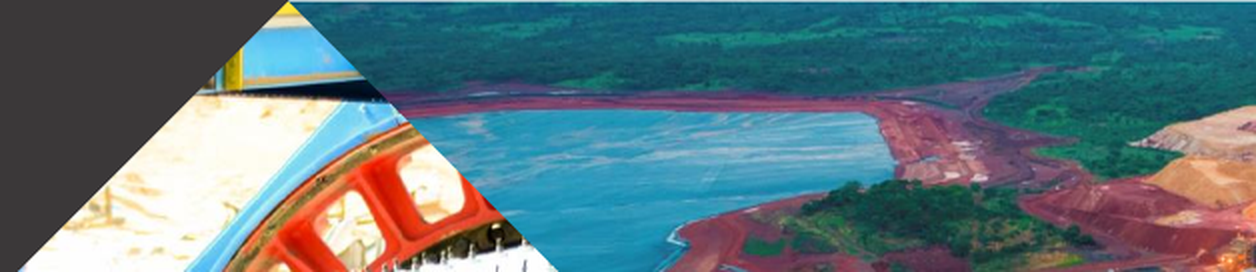
\includegraphics[width=4.2cm]{figures/logo_reminex.png}\\[3mm]
{\normalsize Filiale d'ingénierie du Groupe Managem}\\[1.4cm]

\begin{minipage}{0.9\textwidth}
\centering
\renewcommand{\arraystretch}{1.4}
\begin{tabular}{r l}
\textbf{Élève} & Lina \textsc{Assabane} \\
\textbf{N\textsuperscript{o} d'étudiant} & \rule{3cm}{0.4pt} \\
\textbf{Entité d'accueil} & Reminex --- Groupe Managem \\
\textbf{Service} & Direction Ingénierie / Process Engineering \\
\textbf{Ville} & Casablanca, Maroc \\
\textbf{Période de stage} & du \rule{2cm}{0.4pt} au \rule{2cm}{0.4pt} \\
\textbf{Tuteur d'accueil} & M. Saïd \textsc{Assabane} \\
 & Directeur Adjoint \\
\end{tabular}
\end{minipage}

\vfill
{\footnotesize\color{softgray}Document académique --- restitution du stage de première année}
\end{titlepage}

\pagenumbering{roman}

% ======================================================================
%  2) REMERCIEMENTS
% ======================================================================
\chapter*{Remerciements}
\addcontentsline{toc}{chapter}{Remerciements}
\markboth{Remerciements}{Remerciements}

Au terme de ce stage opérateur, je souhaite exprimer ma reconnaissance à toutes les personnes qui ont rendu cette première immersion dans le monde industriel possible et instructive.

Je remercie tout d'abord M.~Saïd \textsc{Assabane}, Directeur Adjoint et tuteur de mon stage, pour son accueil, sa disponibilité et la confiance qu'il m'a accordée en m'associant à la préparation des rapports d'avancement du projet. Ses explications m'ont permis de comprendre les enjeux concrets d'un chantier industriel.

Je tiens également à remercier les trois ingénieurs qui ont accepté de me consacrer du temps pour me présenter leur métier : M.~Sami \textsc{Sayeh}, pour sa présentation d'ensemble du Groupe Managem et de sa chaîne de valeur~; M.~Houssam \textsc{Benchakroun}, pour son éclairage sur l'organisation interne de Reminex~; et M.~Yassine \textsc{Ouhajjou}, pour son introduction détaillée à l'ingénierie de procédé. Les échanges que j'ai eus avec eux constituent le cœur des apprentissages de ce stage.

Mes remerciements s'adressent plus largement aux équipes de Reminex que j'ai côtoyées, pour leur bienveillance et leur ouverture à mes questions.

Enfin, je remercie l'École Centrale Casablanca et son corps enseignant, qui, à travers ce stage de première année, m'ont offert l'occasion de confronter mes premières connaissances au réel et de préciser mon projet professionnel.

\vspace{1cm}
{\raggedleft\itshape Lina Assabane\par}


% ======================================================================
%  3) GLOSSAIRE / LISTE DES ABRÉVIATIONS
% ======================================================================
\chapter*{Glossaire et liste des abréviations}
\addcontentsline{toc}{chapter}{Glossaire et liste des abréviations}
\markboth{Glossaire et abréviations}{Glossaire et abréviations}

\section*{Sigles et abréviations}

\begin{longtable}{@{}p{2.8cm} p{11.5cm}@{}}
\toprule
\textbf{Sigle} & \textbf{Signification} \\
\midrule
\endfirsthead
\toprule
\textbf{Sigle} & \textbf{Signification} \\
\midrule
\endhead
\bottomrule
\endfoot
BFD & \textit{Block Flow Diagram} --- schéma de procédé par blocs \\
BFS & \textit{Bankable Feasibility Study} --- étude de faisabilité bancable \\
CAPEX & \textit{Capital Expenditure} --- dépenses d'investissement \\
CIL / CIP & \textit{Carbon in Leach} / \textit{Carbon in Pulp} --- procédés d'adsorption de l'or sur charbon actif \\
EPCM & \textit{Engineering, Procurement and Construction Management} \\
HSE & \textit{Health, Safety, Environment} --- hygiène, sécurité, environnement \\
IFC & \textit{Industry Foundation Classes} --- format d'échange des maquettes numériques \\
KPI & \textit{Key Performance Indicator} --- indicateur clé de performance \\
OPEX & \textit{Operating Expenditure} --- dépenses d'exploitation \\
P\&ID & \textit{Piping and Instrumentation Diagram} --- schéma de tuyauterie et d'instrumentation \\
PFD & \textit{Process Flow Diagram} --- schéma de procédé \\
PMC & \textit{Project Management Consultancy} --- assistance à la gestion de projet \\
R\&D & Recherche et Développement \\
ROI & \textit{Return On Investment} --- retour sur investissement \\
ROM & \textit{Run-Of-Mine} --- minerai brut, tel qu'extrait de la mine \\
SID & \textit{Safety In Design} --- sécurité intégrée dès la conception \\
SOP & \textit{Start Of Plant} --- date de démarrage de l'usine \\
\end{longtable}

\section*{Glossaire}

\begin{description}[style=nextline,leftmargin=0pt]
\item[Flowsheet (schéma de procédé)] Représentation de l'enchaînement des opérations unitaires permettant de transformer un minerai brut en produit valorisable (concentré, métal).
\item[Étude d'orientation \textit{(scoping study)}] Première évaluation économique et technique d'un projet, servant à décider de sa poursuite (précision indicative).
\item[Étude de pré-faisabilité] Étude approfondissant plusieurs scénarios techniques et estimant les coûts avec une précision intermédiaire.
\item[Étude de faisabilité] Étude détaillée validant la solution retenue, avec une estimation des coûts de l'ordre de $\pm$\,15--30\,\%, base de la décision d'investissement.
\item[Ingénierie de base \textit{(basic engineering)}] Dimensionnement des principaux équipements et des grands choix techniques du procédé.
\item[Ingénierie de détail \textit{(detailed engineering)}] Production de l'ensemble des plans et documents nécessaires à la construction.
\item[Convoyeur ROM] Convoyeur à bande transportant le minerai brut (\textit{run-of-mine}) depuis la mine vers l'unité de traitement.
\item[Pré-assemblage] Assemblage au sol de sous-ensembles avant leur levage et leur montage en position définitive.
\end{description}


% ======================================================================
%  4) TABLES
% ======================================================================
\microtypesetup{protrusion=false}
\tableofcontents
\listoffigures
\listoftables
\microtypesetup{protrusion=true}
\cleardoublepage

% ======================================================================
%  CORPS DU RAPPORT
% ======================================================================
\pagenumbering{arabic}

\chapter*{Introduction}
\addcontentsline{toc}{chapter}{Introduction}
\markboth{Introduction}{Introduction}

Le stage opérateur de première année n'a pas pour objet de réaliser un travail d'ingénieur, mais de découvrir, de l'intérieur, le fonctionnement d'une organisation et le monde professionnel. C'est dans cet esprit que j'ai effectué mon stage au sein de Reminex, la filiale d'ingénierie du Groupe Managem, rattachée à la Direction Ingénierie.

Je suis arrivée avec une connaissance très générale de l'industrie et une idée encore floue de ce que recouvre concrètement le métier d'ingénieur dans un grand groupe. Mon objectif était donc avant tout d'observer et de comprendre~: comment s'organise une entreprise minière de dimension africaine~? Comment naît et se pilote un projet industriel, depuis l'exploration jusqu'à la production~? Qu'est-ce que l'ingénierie de procédé, dont j'avais surtout entendu parler en cours de manière abstraite~? Et comment les différents métiers d'une même entreprise communiquent-ils entre eux~?

Pour répondre à ces questions, mon stage a reposé sur deux types d'activités complémentaires. D'une part, j'ai contribué, sous la supervision de mon tuteur, à la préparation de rapports hebdomadaires de suivi d'un chantier réel~: l'installation des convoyeurs de la mine de cuivre de Tizert. D'autre part, j'ai bénéficié de plusieurs présentations conduites par des ingénieurs expérimentés, qui m'ont permis de relier ce chantier à une vision plus large de l'ingénierie minière.

Ce rapport rend compte de cette découverte. Il présente d'abord le cadre dans lequel s'est déroulé le stage --- le Groupe Managem et sa filiale Reminex ---, puis la chaîne de valeur minière telle qu'elle m'a été expliquée et les échanges que j'ai eus avec les ingénieurs. Il décrit ensuite les projets que j'ai découverts, le déroulement concret de mon stage et les tâches qui m'ont été confiées. Il se termine par une analyse personnelle de ce que cette expérience m'a apporté et de la manière dont elle a fait évoluer ma vision de l'ingénierie.

Conformément aux consignes de rédaction, les informations factuelles sur le Groupe et ses projets, issues de sources publiques, sont référencées et clairement distinguées de ce que j'ai personnellement observé ou de ce qui m'a été présenté oralement pendant le stage.

\chapter{Présentation du Groupe Managem}

Ce premier chapitre présente le Groupe Managem, entité dont dépend l'entreprise qui m'a accueillie. Les éléments qui suivent proviennent de sources publiques et de la documentation institutionnelle du Groupe~; ils fixent le décor dans lequel s'inscrit mon stage.

\section{Un acteur historique de la mine au Maroc}

Managem est un groupe minier marocain dont les origines remontent à la découverte d'un gisement de cobalt à Bou-Azzer, dans l'Anti-Atlas, à la fin des années 1920~; la première mine du Groupe démarre son activité au début des années 1930~\cite{managem_wiki}. Structuré sous sa forme actuelle dans les années 1990 pour regrouper les activités minières du groupe ONA, il est aujourd'hui coté à la Bourse de Casablanca et rattaché au holding Al~Mada~\cite{managem_wiki}.

Le Groupe couvre l'ensemble de la chaîne minière~: exploration, extraction, traitement (dont l'hydrométallurgie) et commercialisation de métaux de base, de métaux précieux, de cobalt et d'autres substances minérales~\cite{managem_wiki}. Il est présenté par plusieurs sources comme le leader du secteur minier métallique marocain~\cite{afd_potentiel}.

\section{Une présence panafricaine}

Au-delà du Maroc, Managem a développé depuis plus de vingt ans une stratégie d'expansion sur le continent. Le Groupe exploite un ensemble de mines réparties dans plusieurs pays d'Afrique --- notamment la Guinée, le Gabon, la République démocratique du Congo (RDC), le Soudan et, plus récemment, le Sénégal~\cite{afd_potentiel,ecofin_managem}. Cette dimension panafricaine est l'un des traits qui m'ont le plus frappée~: il ne s'agit pas d'une entreprise strictement nationale, mais d'un groupe qui pilote des projets sur des géographies très différentes.

\section{Des minerais stratégiques}

Le portefeuille du Groupe est centré sur plusieurs minerais à forte valeur, dont certains sont dits « stratégiques » car essentiels à la transition énergétique~:

\begin{itemize}
\item le \textbf{cobalt}, historiquement à l'origine du Groupe, avec le gisement de Bou-Azzer, l'un des rares au monde produisant principalement du cobalt~\cite{ecofin_managem}~;
\item l'\textbf{argent}, dont Managem est un producteur majeur en Afrique, notamment via le gisement d'Imiter~\cite{ecofin_managem}~;
\item le \textbf{cuivre}, au cœur de projets d'envergure comme Tizert~;
\item l'\textbf{or}, en forte croissance grâce aux projets ouest-africains (Guinée, Sénégal)~;
\item ainsi que le \textbf{zinc}, le \textbf{plomb} et des minéraux industriels comme la \textbf{fluorine}~\cite{morocco_minerals}.
\end{itemize}

\section{Des projets miniers d'envergure}

Parmi les grands chantiers récents du Groupe, on peut citer la mine d'or de Tri-K en Guinée, le projet cobalt-cuivre de Pumpi en RDC, la mine d'or de Boto au Sénégal et le projet cuprifère de Tizert au Maroc~\cite{ecofin_managem}. Ces deux derniers projets, dont j'ai entendu parler pendant mon stage, sont détaillés au chapitre~\ref{chap:projets}.

\section{Des filiales spécialisées}

Le Groupe fonctionne à travers un ensemble de filiales spécialisées, qui couvrent chacune un maillon de la chaîne. Parmi elles figurent des sociétés d'exploitation minière, une société métallurgique (production d'argent, notamment), des sociétés dédiées à l'or et au cuivre, et --- ce qui me concerne directement --- \textbf{Reminex}, la filiale d'ingénierie et de recherche du Groupe, présentée au chapitre suivant.

\begin{presente}
\textbf{Ce que je retiens de ce cadre.} Avant ce stage, je voyais « la mine » comme une simple activité d'extraction. J'ai compris que Managem est en réalité un groupe intégré, qui va de la recherche du gisement jusqu'à la vente du métal, sur plusieurs continents, et qui s'appuie pour cela sur des filiales aux métiers très différents.
\end{presente}

\chapter{Présentation de Reminex}
\label{chap:reminex}

Reminex est l'entité au sein de laquelle j'ai effectué mon stage. Les informations de ce chapitre s'appuient principalement sur la documentation de présentation de l'entreprise (\textit{Expertise \& Capabilities})~\cite{reminex_capabilities} et sur les explications qui m'ont été données pendant le stage.

\section{La filiale d'ingénierie du Groupe Managem}

Reminex est la filiale d'ingénierie et de recherche du Groupe Managem. Sa vocation est d'accompagner les projets miniers du Groupe --- et de clients extérieurs --- depuis l'exploration jusqu'à la mise en production, puis au-delà, pendant l'exploitation. Elle réunit, d'après sa documentation, plus de quatre-vingts spécialistes et revendique plusieurs dizaines d'années d'expérience cumulée en projets et en opérations minières, une dizaine de brevets et un large portefeuille de procédés développés en interne~\cite{reminex_capabilities}.

Ce positionnement est particulier~: parce qu'elle appartient à un groupe qui exploite lui-même des mines, Reminex combine une culture d'ingénierie « de bureau » et une culture d'exploitation « de terrain ». C'est un point qui revient souvent dans sa communication et que les ingénieurs m'ont confirmé~: concevoir en connaissant les contraintes réelles de l'exploitation.

\section{Trois missions : créer, livrer, améliorer}

L'entreprise résume sa mission autour de trois verbes, qui structurent aussi la manière dont elle intervient sur un projet~\cite{reminex_capabilities}~:

\begin{center}
\begin{tikzpicture}[
  node distance=6mm,
  mission/.style={rectangle, rounded corners, draw=reminexorange!80, fill=reminexorange!12,
    text width=3.3cm, minimum height=1.6cm, align=center, font=\small},
  arr/.style={-{Stealth[length=3mm]}, reminexorange!80, line width=1pt}]
\node[mission] (c) {\textbf{Créer}\\[2pt]\scriptsize concevoir des solutions et des \textit{flowsheets} pour valoriser les gisements};
\node[mission, right=of c] (d) {\textbf{Livrer}\\[2pt]\scriptsize conception, ingénierie et exécution du projet jusqu'à sa réussite};
\node[mission, right=of d] (i) {\textbf{Améliorer}\\[2pt]\scriptsize accompagner l'exploitation pour améliorer durablement l'actif};
\draw[arr] (c) -- (d);
\draw[arr] (d) -- (i);
\end{tikzpicture}
\captionof{figure}{Les trois missions de Reminex (d'après la documentation de l'entreprise~\cite{reminex_capabilities}).}
\label{fig:missions}
\end{center}

Autrement dit, l'entreprise ne s'arrête pas à la remise des plans~: elle intervient en amont (études, conception du procédé) et en aval (mise en service, optimisation de l'usine en production).

\section{Un éventail de disciplines d'ingénierie}

La conception d'une usine minière mobilise simultanément de nombreuses spécialités. Reminex dispose en interne d'une équipe pluridisciplinaire couvrant notamment les disciplines suivantes~\cite{reminex_capabilities}~:

\begin{center}
\renewcommand{\arraystretch}{1.25}
\begin{tabular}{@{}p{3.4cm} p{10.5cm}@{}}
\toprule
\textbf{Discipline} & \textbf{Rôle dans le projet} \\
\midrule
Procédé (\textit{Process}) & Définit le \textit{flowsheet}, les bilans matière et les conditions de fonctionnement. \\
Mécanique & Choix et dimensionnement des équipements (concasseurs, pompes, convoyeurs\ldots). \\
Génie civil & Fondations, ouvrages en béton, terrassements. \\
Structure & Charpentes métalliques supportant les équipements. \\
Tuyauterie (\textit{Piping}) & Réseaux de fluides reliant les équipements. \\
Instrumentation & Capteurs et boucles de mesure/régulation. \\
Électricité & Distribution et motorisation. \\
Environnement & Gestion des rejets, de l'eau, des stériles. \\
Gestion de projet & Planning, coûts, coordination des disciplines. \\
\bottomrule
\end{tabular}
\captionof{table}{Principales disciplines d'ingénierie de Reminex.}
\label{tab:disciplines}
\end{center}

La particularité, que j'ai découverte pendant le stage, est que ces disciplines ne travaillent pas les unes après les autres mais \emph{ensemble}~: un choix de procédé impose une structure, qui impose une tuyauterie, qui impose une alimentation électrique, etc. La coordination entre elles est un métier à part entière (la gestion de projet).

\section{Un accompagnement « de la mine au produit »}

Enfin, Reminex décrit son offre comme un accompagnement continu couvrant tout le cycle d'un projet minier, « de la fosse au produit »~\cite{reminex_capabilities}~: exploration et caractérisation, développement du \textit{flowsheet}, ingénierie et conception, gestion de la construction (jusqu'à l'\sig{epcm}), mise en service et démarrage, puis excellence opérationnelle pendant la production. Ce continuum est important pour comprendre la suite du rapport~: chaque projet du Groupe se situe à un moment précis de ce cycle.

\chapter{La chaîne de valeur minière}
\label{chap:chaine}

L'une des présentations les plus structurantes de mon stage a été celle de M.~Sami~\textsc{Sayeh}, qui m'a exposé l'organisation générale du Groupe et la « chaîne de valeur » minière. Ce chapitre restitue, avec mes mots, ce qui m'a été expliqué lors de cet échange~; il s'agit donc d'une source orale, complétée par mes notes.

\section{Du gisement au métal : une succession d'étapes}

M.~Sayeh m'a d'abord fait comprendre qu'un projet minier n'est pas un acte unique mais une longue succession d'étapes, chacune conditionnant la suivante. Je les ai schématisées ainsi~:

\begin{center}
\begin{tikzpicture}[
  node distance=2.1mm,
  vnode/.style={rectangle, rounded corners=2pt, draw=centralegreen!70, fill=centralegreen!8,
    text width=5.6cm, minimum height=6mm, align=center, font=\small},
  arr/.style={-{Stealth[length=2.5mm]}, centralegreen!70, line width=0.9pt}]
\node[vnode] (s1) {Exploration};
\node[vnode, below=of s1] (s2) {Géologie};
\node[vnode, below=of s2] (s3) {Estimation des ressources};
\node[vnode, below=of s3] (s4) {Conception de la mine \textit{(mine design)}};
\node[vnode, below=of s4] (s5) {Extraction (exploitation minière)};
\node[vnode, below=of s5] (s6) {Transport du minerai};
\node[vnode, below=of s6] (s7) {Traitement du minerai};
\node[vnode, below=of s7] (s8) {Métallurgie};
\node[vnode, below=of s8] (s9) {Commercialisation};
\node[vnode, below=of s9] (s10) {Amélioration continue};
\foreach \a/\b in {s1/s2,s2/s3,s3/s4,s4/s5,s5/s6,s6/s7,s7/s8,s8/s9,s9/s10}
  \draw[arr] (\a) -- (\b);
\end{tikzpicture}
\captionof{figure}{La chaîne de valeur minière telle qu'elle m'a été présentée.}
\label{fig:chaine}
\end{center}

Ce qui m'a marquée, c'est que la valeur se construit progressivement~: on part d'une simple hypothèse géologique et on aboutit, au bout de la chaîne, à un métal vendable. Chaque étape « ajoute » de la connaissance ou de la transformation, et une erreur en amont (par exemple une mauvaise estimation des ressources) se paie très cher en aval.

\section{Indicateurs et logique de traitement}

M.~Sayeh a insisté sur quelques \sig{kpi} globaux qui suivent le minerai tout au long de la chaîne, en particulier le \textbf{tonnage}, la \textbf{teneur} (concentration en métal) et le \textbf{rendement} de récupération. C'est la combinaison de ces trois grandeurs qui détermine la quantité de métal réellement produite.

Il m'a aussi montré que le \emph{procédé de traitement dépend du métal visé}. À partir de mes notes, j'ai retenu trois grandes familles~:

\begin{itemize}
\item les \textbf{métaux précieux} (or, argent) sont généralement traités par cyanuration, avec des procédés d'adsorption sur charbon actif de type \sig{cil}/\sig{cip}, aboutissant à un doré ou à un concentré~;
\item le \textbf{cuivre} est concentré par \textbf{flottation} avant traitement (projets tels que Tizert, Akka, Guemassa)~;
\item le \textbf{cobalt} relève d'une voie \textbf{hydrométallurgique}.
\end{itemize}

Je n'ai pas cherché à maîtriser ces procédés en détail --- ce n'était pas l'objet du stage --- mais à comprendre l'idée générale~: à chaque minerai correspond une « recette » de traitement, et c'est précisément le rôle de l'ingénierie de procédé de définir cette recette.

\section{Où intervient Reminex ?}

La dernière chose que M.~Sayeh m'a aidée à situer, c'est la place de Reminex dans cette chaîne. Reminex n'exploite pas la mine~: elle intervient surtout sur les maillons de \emph{conception et de réalisation}. Concrètement~:

\begin{itemize}
\item en amont, elle contribue à la \textbf{caractérisation} du minerai et au \textbf{développement du \textit{flowsheet}} (par son centre de R\&D)~;
\item au cœur du projet, elle réalise l'\textbf{ingénierie} (transformer le \textit{flowsheet} en usine) et pilote la \textbf{construction}~;
\item en aval, elle accompagne la \textbf{mise en service} et l'\textbf{amélioration} des installations en production.
\end{itemize}

Autrement dit, Reminex est l'entité qui fait passer un projet du « laboratoire » à « l'usine ». Cette idée, esquissée ici, est développée dans les échanges avec les ingénieurs (chapitre~\ref{chap:ingenieurs}).

\chapter{Échanges avec les ingénieurs}
\label{chap:ingenieurs}

Le cœur de mon apprentissage a reposé sur des échanges avec trois ingénieurs occupant des fonctions de direction adjointe au sein de Reminex. Chacun m'a présenté un aspect différent du métier. Les développements ci-dessous restituent ce qui m'a été exposé lors de ces discussions~; il s'agit de sources orales, appuyées sur les notes que j'ai prises.

% ---------------------------------------------------------------------
\section{M. Sami Sayeh --- vision d'ensemble du Groupe}

M.~Sami~\textsc{Sayeh} m'a offert la première mise en perspective de mon stage. C'est lui qui m'a présenté le Groupe Managem et la chaîne de valeur minière détaillée au chapitre~\ref{chap:chaine}.

Au-delà de ce panorama, il a surtout mis en évidence les \textbf{liens entre trois grands mondes} qui doivent constamment dialoguer~: l'\textbf{exploration} (qui découvre et caractérise le gisement), l'\textbf{ingénierie} (qui conçoit l'usine et les infrastructures) et les \textbf{opérations} (qui exploitent). J'ai retenu que ces trois fonctions ne se succèdent pas simplement dans le temps~: elles s'informent mutuellement. L'ingénierie a besoin des données de l'exploration~; les opérations remontent vers l'ingénierie des retours de terrain qui nourrissent l'amélioration continue. Cette circulation d'informations entre métiers est une idée qui reviendra dans tout le rapport.

% ---------------------------------------------------------------------
\section{M. Houssam Benchakroun --- l'organisation de Reminex}

M.~Houssam~\textsc{Benchakroun} m'a présenté l'\textbf{organisation interne de Reminex}. À partir de ses explications et de mes notes, j'ai reconstitué le schéma suivant~:

\begin{center}
\begin{tikzpicture}[
  box/.style={rectangle, rounded corners=2pt, draw=darkslate!60, fill=darkslate!5,
    text width=3.1cm, minimum height=9mm, align=center, font=\small},
  head/.style={rectangle, rounded corners=2pt, draw=reminexorange!80, fill=reminexorange!12,
    text width=3.4cm, minimum height=9mm, align=center, font=\small\bfseries},
  sub/.style={rectangle, rounded corners=2pt, draw=centralegreen!60, fill=centralegreen!7,
    text width=3.4cm, minimum height=8mm, align=center, font=\footnotesize},
  arr/.style={-{Stealth[length=2.5mm]}, darkslate!60, line width=0.8pt}]
\node[head] (rem) {Reminex\\\scriptsize recherche minière \& exploration};
\node[box, below left=12mm and 6mm of rem] (ing) {Ingénierie};
\node[box, below=12mm of rem] (rd) {Centre R\&D};
\node[box, below right=12mm and 6mm of rem] (exp) {Exploration minière};
\draw[arr] (rem) -- (ing);
\draw[arr] (rem) -- (rd);
\draw[arr] (rem) -- (exp);
\node[sub, below=8mm of rd] (car) {\textcircled{1}~Caractérisation};
\node[sub, below=6mm of car] (pro) {\textcircled{2}~Procédé / \textit{flowsheet}};
\draw[arr] (rd) -- (car);
\draw[arr] (car) -- (pro);
\draw[arr, dashed] (rd.west) to[out=180,in=90] (ing.north);
\end{tikzpicture}
\captionof{figure}{Organisation interne de Reminex reconstituée d'après la présentation de M.~Benchakroun.}
\label{fig:org_reminex}
\end{center}

Reminex s'articule ainsi autour de trois pôles principaux~: l'\textbf{Ingénierie}, un \textbf{centre de Recherche \& Développement} et l'\textbf{Exploration minière}. M.~Benchakroun a particulièrement détaillé le rôle du centre de R\&D, qui réalise notamment~:

\begin{itemize}
\item la \textbf{caractérisation} du minerai (comprendre sa composition et son comportement)~;
\item le \textbf{développement du procédé et du \textit{flowsheet}} (définir comment le traiter).
\end{itemize}

Ce qui m'a paru important, c'est la \emph{collaboration} entre ces pôles~: le centre de R\&D fournit à l'Ingénierie le \textit{flowsheet} et les données que celle-ci va « industrialiser », tandis que l'Exploration alimente l'ensemble en connaissance du gisement. On retrouve, à l'échelle de Reminex, la même logique d'interdépendance que celle décrite par M.~Sayeh.

% ---------------------------------------------------------------------
\section{M. Yassine Ouhajjou --- l'ingénierie de procédé}

M.~Yassine~\textsc{Ouhajjou}, qui travaille en ingénierie de procédé, m'a fait la présentation la plus technique de mon stage. Son fil conducteur tenait en une phrase que j'ai notée telle quelle~: \textit{« transformer le \textit{flowsheet} en usine »}.

\subsection{Faire dialoguer toutes les disciplines}

Il a d'abord montré que passer d'un schéma de procédé à une usine réelle nécessite de mobiliser, autour du procédé, l'ensemble des disciplines~: génie civil, structure, mécanique, tuyauterie (\textit{piping}), instrumentation, ainsi que la démarche de sécurité intégrée dès la conception (\sig{sid}, \textit{Safety In Design}) et la prise en compte de l'environnement. Le procédé est au centre, mais il ne « tient debout » que grâce à toutes ces spécialités.

\subsection{Les documents clés de l'ingénierie}

M.~Ouhajjou a ensuite introduit les grands \textbf{livrables} qui décrivent progressivement l'usine, du plus général au plus détaillé~:

\begin{center}
\begin{tikzpicture}[
  doc/.style={rectangle, rounded corners=2pt, draw=reminexorange!80, fill=reminexorange!10,
    text width=2.5cm, minimum height=1.4cm, align=center, font=\footnotesize},
  arr/.style={-{Stealth[length=2.5mm]}, reminexorange!80, line width=1pt}]
\node[doc] (bfd) {\textbf{BFD}\\\scriptsize schéma par blocs};
\node[doc, right=8mm of bfd] (pfd) {\textbf{PFD}\\\scriptsize schéma de procédé};
\node[doc, right=8mm of pfd] (pid) {\textbf{P\&ID}\\\scriptsize tuyauterie \& instrumentation};
\node[doc, right=8mm of pid] (ds) {\textbf{Datasheets}\\\scriptsize fiches techniques équipements};
\draw[arr] (bfd) -- (pfd);
\draw[arr] (pfd) -- (pid);
\draw[arr] (pid) -- (ds);
\end{tikzpicture}
\captionof{figure}{Du plus général au plus détaillé~: les principaux livrables présentés par M.~Ouhajjou.}
\label{fig:documents}
\end{center}

Le \sig{bfd} donne la vue d'ensemble par grands blocs~; le \sig{pfd} précise les flux du procédé~; le \sig{pid} descend au niveau des tuyauteries et de l'instrumentation~; enfin les \textit{datasheets} spécifient chaque équipement. J'ai trouvé cette progression très éclairante~: elle illustre concrètement comment une idée abstraite devient un objet constructible.

\subsection{Le coût et la décision d'investir}

Un projet ne se juge pas seulement techniquement mais aussi \textbf{économiquement}. M.~Ouhajjou m'a présenté deux notions centrales~:

\begin{itemize}
\item le \sig{capex} (\textit{Capital Expenditure}), c'est-à-dire le coût d'investissement pour construire l'usine~;
\item l'\sig{opex} (\textit{Operating Expenditure}), c'est-à-dire le coût d'exploitation, une fois l'usine en marche (réactifs, énergie, main-d'œuvre\ldots).
\end{itemize}

La rentabilité se mesure ensuite par le retour sur investissement (\sig{roi}). Je précise que je n'ai réalisé \emph{aucun calcul} de ce type~: ces notions m'ont été expliquées pour que je comprenne la logique de décision, et non pour être mises en pratique.

\subsection{La maturation d'un projet par étapes}

Enfin, M.~Ouhajjou a insisté sur le fait qu'un projet minier ne se conçoit pas d'un seul coup~: il « mûrit » par étapes, chacune de plus en plus précise et de plus en plus coûteuse à produire. J'ai retenu l'enchaînement suivant~:

\begin{center}
\begin{tikzpicture}[
  ph/.style={rectangle, rounded corners=2pt, draw=centralegreen!70, fill=centralegreen!8,
    text width=2.55cm, minimum height=1.5cm, align=center, font=\scriptsize},
  arr/.style={-{Stealth[length=2.5mm]}, centralegreen!70, line width=1pt}]
\node[ph] (o) {\textbf{Étude\\d'orientation}\\\textit{(scoping)}\\précision indicative};
\node[ph, right=6mm of o] (pf) {\textbf{Pré-\\faisabilité}\\plusieurs scénarios};
\node[ph, right=6mm of pf] (f) {\textbf{Faisabilité}\\solution retenue\\($\approx\pm$\,30\,\%)};
\node[ph, right=6mm of f] (b) {\textbf{Ingénierie\\de base}\\dimensionnement};
\node[ph, right=6mm of b] (d) {\textbf{Ingénierie\\de détail}\\plans de construction};
\draw[arr] (o) -- (pf);
\draw[arr] (pf) -- (f);
\draw[arr] (f) -- (b);
\draw[arr] (b) -- (d);
\end{tikzpicture}
\captionof{figure}{Maturation d'un projet, de l'étude d'orientation à l'ingénierie de détail.}
\label{fig:maturation}
\end{center}

Ce séquencement m'a permis de comprendre une idée essentielle~: on n'investit massivement qu'après avoir progressivement réduit l'incertitude. La précision des estimations augmente à mesure qu'on avance dans les études, et c'est seulement à la fin que l'on engage la construction. C'est, en quelque sorte, le passage « du laboratoire à la production industrielle » que M.~Sayeh avait évoqué au début du stage.

\chapter{Deux grands projets découverts}
\label{chap:projets}

Pendant mon stage, deux projets du Groupe ont particulièrement retenu mon attention~: la mine d'or de Boto, au Sénégal, et le projet cuprifère de Tizert, au Maroc, sur lequel a porté le travail de suivi auquel j'ai été associée. Les données chiffrées de ce chapitre proviennent de sources publiques et sont référencées~; ce que j'ai personnellement observé est signalé comme tel.

% ---------------------------------------------------------------------
\section{Boto --- une mine d'or au Sénégal}

\subsection{Localisation et objectifs}

Le projet Boto est situé dans la région de Kédougou, à l'est du Sénégal, près des frontières du Mali et de la Guinée, dans une zone géologique (le \textit{Senegalo-Malian Shear Zone}) qui abrite plusieurs gisements aurifères de classe mondiale~\cite{managem_boto}. Il s'agit d'une mine d'\textbf{or} à ciel ouvert, acquise par Managem en 2023 auprès de la société canadienne IAMGOLD, le Groupe en détenant 90\,\% aux côtés de l'État sénégalais~\cite{allafrica_boto}.

\subsection{Un investissement majeur et un statut récent}

Boto représente un investissement de l'ordre de 350~millions d'euros, ce qui en fait l'un des plus importants développements miniers du Sénégal~\cite{managem_boto,northafrica_boto}. Le projet vise une production moyenne d'environ 160\,000~onces d'or par an sur ses trois premières années, pour des réserves estimées à près de 1,8~million d'onces et une durée de vie d'une douzaine d'années~\cite{managem_boto}. La mine s'appuie sur une usine de traitement et des infrastructures dédiées (centrale électrique, digues, base-vie, piste d'atterrissage, réseau routier)~\cite{northafrica_boto}.

Le fait le plus marquant est que Boto est passé, très récemment, du stade de la construction à celui de la \textbf{production}~: la première coulée d'or a eu lieu le 2~septembre 2025~\cite{managem_boto}. Le projet est donc, à l'échelle du Groupe, un exemple actuel de passage réussi « du chantier à l'exploitation ».

\subsection{Importance et défis d'ingénierie}

Pour Managem, Boto consolide la stratégie aurifère du Groupe en Afrique de l'Ouest et renforce son positionnement de producteur régional d'or~\cite{allafrica_boto}. Sur le plan de l'ingénierie, un tel projet illustre bien les enjeux évoqués par les ingénieurs~: construire, dans une zone isolée, non seulement une usine mais tout un écosystème (énergie, eau, logistique, hébergement), et le faire dans des délais maîtrisés. Je n'ai pas travaillé sur ce projet~; il m'a servi de \emph{point de repère} pour comprendre ce qu'est un projet minier arrivé à maturité.

% ---------------------------------------------------------------------
\section{Tizert --- le projet cuprifère}

\subsection{Un projet stratégique pour le cuivre marocain}

Le projet Tizert est situé dans l'Anti-Atlas occidental, à environ 65~km de Taroudant, sur la bordure nord de la boutonnière d'Igherm~\cite{managem_tizert}. C'est l'un des plus importants gisements de \textbf{cuivre} (Cu-Ag) du Maroc, exploité en fosse et en souterrain. Le projet représente un investissement de l'ordre de 440~millions de dollars et vise une capacité de production de l'ordre de 100 à 120~kilotonnes de concentré de cuivre par an, pour une durée de vie d'environ 17 à 18~ans~\cite{managem_tizert}. Comme Boto, Tizert est entré en production commerciale en 2025, avec les premières ventes de concentré au quatrième trimestre~\cite{managem_tizert}.

L'importance de Tizert dépasse le seul cadre du Groupe~: sa production doit couvrir une part significative des besoins nationaux en cuivre, métal essentiel à la transition énergétique~\cite{managem_tizert}. Les études de faisabilité du projet ont d'ailleurs mobilisé Reminex aux côtés de cabinets d'ingénierie de renommée internationale~\cite{managem_tizert}, ce qui donne un sens très concret au rôle de la filiale décrit précédemment.

\subsection{L'installation des convoyeurs ROM}

C'est sur un chantier précis de Tizert que j'ai été associée à un travail de suivi~: l'\textbf{installation des convoyeurs ROM} (\textit{Run-Of-Mine}), c'est-à-dire les convoyeurs à bande qui acheminent le minerai brut vers l'unité de traitement. D'après les documents de suivi que j'ai contribué à mettre en forme, ce chantier porte sur deux lignes de convoyage identifiées par leur numéro de plan~:

\begin{itemize}
\item le \textbf{convoyeur principal (Plan~1005)}, une ligne aérienne suspendue (tronçons, tour d'escalier, structure treillis, pylônes de support)~;
\item le \textbf{convoyeur du tunnel (Plan~1037)}, une ligne en galerie.
\end{itemize}

L'avancement est suivi selon trois jalons cumulatifs --- inventaire, pré-assemblage et montage --- et fait l'objet d'un tableau de bord hebdomadaire (indicateurs de sécurité, tonnage réalisé, courbes d'avancement, planning). Un exemple de ce rapport, dont j'ai contribué à la mise en forme, est reproduit en annexe~\ref{ann:rapport} \emph{à titre d'illustration du format de reporting}, et non comme un travail dont je serais l'auteur.

\begin{presente}
\textbf{Mon rôle, précisément.} Je n'ai pas conçu ni dimensionné ces convoyeurs. J'ai aidé à \emph{préparer} les rapports d'avancement~: collecter et organiser les informations transmises par les équipes de montage, mettre en forme les tableaux et les figures, et produire un document professionnel. Ce travail, réalisé sous la supervision de mon tuteur, est détaillé au chapitre~\ref{chap:stage}.
\end{presente}

\chapter{Le déroulement de mon stage}
\label{chap:stage}

Ce chapitre décrit concrètement ce que j'ai fait pendant mon stage. Comme il s'agit d'un stage opérateur, mes tâches relevaient de l'assistance et de l'observation plutôt que de la production d'ingénierie~; je m'attache donc à décrire honnêtement mon rôle réel, les difficultés rencontrées et la manière dont je les ai gérées.

\section{Contribuer à la préparation des rapports d'avancement}

Ma principale contribution a consisté à assister mon tuteur, M.~Saïd~\textsc{Assabane}, Directeur Adjoint, dans la \textbf{préparation des rapports hebdomadaires} de suivi du chantier des convoyeurs de Tizert (chapitre~\ref{chap:projets}). Concrètement, mes tâches ont été les suivantes~:

\begin{itemize}
\item \textbf{collecter} les informations transmises par les équipes de montage et par l'entreprise (avancement, faits marquants, points de vigilance)~;
\item \textbf{organiser} ces informations techniques de façon claire et cohérente d'une semaine à l'autre~;
\item \textbf{mettre en forme} des tableaux (indicateurs d'avancement, tonnages) et intégrer des figures (photos de chantier, courbes)~;
\item \textbf{rédiger et mettre en page} le document sous \LaTeX, afin d'obtenir un rendu professionnel et homogène.
\end{itemize}

Je tiens à être précise sur ce point~: \emph{je n'étais pas l'auteure de ces rapports}. J'ai contribué à leur préparation et à leur mise en forme, sous la supervision de mon tuteur, qui en validait le contenu. Mon apport se situait donc dans l'\textbf{organisation} et la \textbf{présentation} de l'information, non dans l'analyse technique du chantier.

\paragraph{Difficultés rencontrées et solutions.} Ce travail, en apparence simple, m'a confrontée à plusieurs difficultés que j'ai dû apprendre à gérer~:
\begin{itemize}
\item Le \textbf{vocabulaire technique} (pré-assemblage, tronçons \textit{Gantry}, pylônes de support, jalons d'avancement) m'était au départ inconnu. Je me suis constitué un petit lexique personnel et je n'ai pas hésité à demander des clarifications, ce qui a nourri le glossaire de ce rapport.
\item Les informations arrivaient de \textbf{sources multiples} et pas toujours homogènes. J'ai appris à recouper les données et à privilégier une structure stable de rapport, reprise et actualisée chaque semaine, plutôt que de tout refaire à chaque fois.
\item La \textbf{mise en page \LaTeX} de tableaux et de figures a demandé de la rigueur~; les difficultés techniques m'ont poussée à progresser dans cet outil, ce qui constitue l'un des apports concrets du stage.
\end{itemize}

\section{Assister aux échanges techniques}

Mon stage a également comporté une part importante d'\textbf{écoute et d'observation}, à travers les présentations conduites par les ingénieurs (chapitre~\ref{chap:ingenieurs}). Ces échanges m'ont permis de comprendre, sans avoir à les pratiquer moi-même~:

\begin{itemize}
\item l'ingénierie de procédé (comment transformer un \textit{flowsheet} en usine)~;
\item la gestion de projet (études par étapes, maîtrise des coûts, planning)~;
\item l'organisation industrielle d'un grand groupe minier~;
\item les grands principes de l'ingénierie minière.
\end{itemize}

Mon attitude, dans ce contexte, a consisté à préparer des questions, à prendre des notes structurées et à reformuler ce que j'avais compris pour le vérifier --- une posture d'apprentissage que je crois avoir développée au fil des semaines.

\section{Observer la communication entre les métiers}

Enfin, ce stage m'a offert un poste d'observation privilégié sur la \textbf{communication entre les différents métiers} de l'ingénierie. En suivant le chantier et les échanges, j'ai constaté que la réalisation d'un ouvrage aussi « simple » en apparence qu'un convoyeur suppose la coordination de nombreuses disciplines~:

\begin{center}
\begin{tikzpicture}[
  disc/.style={rectangle, rounded corners=2pt, draw=darkslate!55, fill=darkslate!5,
    minimum width=2.4cm, minimum height=7mm, align=center, font=\footnotesize},
  hub/.style={circle, draw=reminexorange!80, fill=reminexorange!12,
    minimum size=2cm, align=center, font=\small\bfseries},
  arr/.style={{Stealth[length=2mm]}-{Stealth[length=2mm]}, softgray, line width=0.6pt}]
\node[hub] (proj) {Gestion\\de projet};
\node[disc, above left=10mm and 14mm of proj] (proc) {Procédé};
\node[disc, above=12mm of proj] (meca) {Mécanique};
\node[disc, above right=10mm and 14mm of proj] (civil) {Génie civil};
\node[disc, below left=10mm and 14mm of proj] (pip) {Tuyauterie};
\node[disc, below=12mm of proj] (instr) {Instrumentation};
\node[disc, below right=10mm and 14mm of proj] (constr) {Construction};
\foreach \d in {proc,meca,civil,pip,instr,constr}
  \draw[arr] (proj) -- (\d);
\end{tikzpicture}
\captionof{figure}{La gestion de projet coordonne le dialogue entre les disciplines.}
\label{fig:coordination}
\end{center}

J'ai notamment observé, à travers les rapports de chantier, comment un problème apparemment mineur --- par exemple une difficulté d'identification des pièces entre les plans d'assemblage et les maquettes numériques --- pouvait ralentir tout un chantier et nécessitait une coordination renforcée entre les intervenants. Cette interdépendance des métiers est sans doute l'un des enseignements les plus concrets de mon stage.

\chapter{Les apports du stage}
\label{chap:apports}

Au-delà des tâches réalisées, ce stage m'a apporté un ensemble d'enseignements que je regroupe ici en trois familles~: des connaissances sur le métier d'ingénieur, des compétences pratiques, et une meilleure compréhension du fonctionnement d'une organisation.

\section{Comprendre l'ingénierie avant d'y entrer}

Le premier apport, et le plus précieux, est d'ordre presque « culturel ». Avant ce stage, l'ingénierie était pour moi une notion abstraite. J'en repars avec des repères concrets~:

\begin{itemize}
\item je sais désormais ce que recouvrent des documents comme le \sig{pfd} ou le \sig{pid}, et pourquoi ils sont indispensables~: ils constituent le langage commun qui permet aux disciplines de se comprendre et de construire la même usine~;
\item je comprends la logique économique d'un projet, à travers le \sig{capex} et l'\sig{opex}, et l'idée qu'un projet se décide autant sur des critères financiers que techniques~;
\item j'ai saisi qu'un projet industriel se construit \textbf{par étapes} (de l'étude d'orientation à l'ingénierie de détail), en réduisant progressivement l'incertitude avant d'engager les investissements lourds.
\end{itemize}

Le fait de découvrir cette « grammaire » de l'ingénierie \emph{avant} d'entrer dans le cycle ingénieur me paraît être un avantage réel pour la suite de ma formation~: les cours à venir auront désormais un ancrage concret.

\section{Des compétences pratiques}

Le stage m'a aussi permis d'acquérir ou de renforcer des compétences directement transférables~:

\begin{itemize}
\item la \textbf{rédaction de documents professionnels}~: structurer une information technique, la hiérarchiser, la rendre lisible pour un lecteur pressé~;
\item la \textbf{maîtrise de \LaTeX}~: mise en page de tableaux, intégration de figures, production de documents soignés et homogènes --- une compétence que je réinvestis d'ailleurs dans ce rapport~;
\item la capacité à \textbf{recouper et organiser} des informations issues de plusieurs sources, dans un cadre où la fiabilité et la clarté priment.
\end{itemize}

\section{Le fonctionnement d'une organisation}

Enfin, ce stage a été une véritable leçon d'\textbf{organisation industrielle}. J'en retiens surtout~:

\begin{itemize}
\item l'importance de la \textbf{communication entre les métiers}~: aucune discipline ne travaille isolément, et la coordination est un métier en soi (la gestion de projet)~;
\item la centralité de la \textbf{sécurité} (\sig{hse})~: dans les rapports de chantier, les indicateurs de sécurité figurent \emph{avant} les indicateurs d'avancement, ce qui traduit une véritable hiérarchie des priorités~;
\item la valeur du \textbf{travail d'équipe} et de l'\textbf{interdisciplinarité}~: la réussite d'un projet dépend moins de performances individuelles que de la qualité des interfaces entre les personnes et les métiers.
\end{itemize}

Ces enseignements dépassent le cadre strict de l'industrie minière et me semblent transposables à la plupart des environnements de projet.

\chapter{Analyse personnelle}
\label{chap:analyse}

Cette dernière partie propose un regard critique et personnel sur mon stage~: ce qui m'a surprise, ce qui a été difficile, et la manière dont cette expérience a fait évoluer ma vision de l'ingénierie et mon projet professionnel.

\section{Ce qui m'a surprise}

Trois choses m'ont particulièrement étonnée. D'abord, l'\textbf{ampleur} et l'intégration du Groupe~: je découvrais que « la mine » n'est pas une activité isolée mais un système complet, de l'exploration à la commercialisation, déployé à l'échelle de tout un continent.

Ensuite, la \textbf{place de l'écrit et du document}. J'imaginais l'ingénierie comme une affaire de calculs~; j'ai réalisé qu'elle repose tout autant sur des documents structurés (\sig{pfd}, \sig{pid}, \textit{datasheets}, rapports) qui font circuler l'information entre les métiers. La qualité de la communication est une compétence d'ingénieur à part entière.

Enfin, la \textbf{part de l'incertitude et de la décision}. J'ai été surprise de constater qu'un projet n'est jamais « certain » d'emblée~: on avance par étapes, en affinant progressivement les estimations avant d'oser investir. L'ingénierie n'est pas seulement technique, elle est aussi une gestion du risque.

\section{Ce qui a été difficile}

La principale difficulté a été, au début, de me sentir \textbf{légitime} dans un environnement d'experts, avec un vocabulaire que je ne maîtrisais pas. J'ai dû apprendre à assumer mon statut d'apprenante~: poser des questions, reconnaître ce que je ne comprenais pas, et transformer cette curiosité en moteur plutôt qu'en gêne.

Une seconde difficulté, plus technique, a été de \textbf{rester rigoureuse} dans la mise en forme d'informations que je ne comprenais pas toujours entièrement. J'ai appris qu'on peut contribuer utilement à un travail --- en l'organisant et en le présentant --- même sans en maîtriser tous les aspects techniques, à condition de rester honnête sur son propre périmètre.

\section{Points forts et limites du stage}

Le principal \textbf{point fort} de ce stage a été la \emph{qualité de l'encadrement et des échanges}~: le temps que les ingénieurs m'ont consacré a transformé une simple observation en véritable apprentissage. J'ai également apprécié de pouvoir relier un chantier réel (Tizert) à une vision d'ensemble.

Sa principale \textbf{limite} tient à la nature même d'un stage opérateur~: je n'ai pas pu mettre en pratique de compétences d'ingénierie proprement dites, ni approfondir un sujet technique. Mais ce n'était pas l'objectif~: ce stage était une \emph{découverte}, et il a pleinement rempli ce rôle. Il me manque encore, pour un futur stage, une réelle mise en pratique technique --- ce sera justement l'objet de mes prochaines expériences.

\section{L'évolution de ma vision de l'ingénierie}

Ce stage a nettement fait évoluer ma représentation du métier. Je pensais que l'ingénieur était avant tout un « résolveur de problèmes techniques » isolé~; j'en repars avec l'image d'un professionnel qui \textbf{coordonne}, qui \textbf{communique} et qui \textbf{décide} dans l'incertitude, au sein d'un collectif de disciplines. La dimension humaine et organisationnelle de l'ingénierie m'apparaît désormais aussi importante que sa dimension technique.

\section{Impact sur mon projet professionnel}

Sur le plan de mon orientation, cette expérience a \textbf{renforcé un intérêt} que je pressentais pour l'\textbf{ingénierie industrielle} et la \textbf{gestion de projet}. Ce qui m'a le plus attirée n'est pas tel ou tel procédé, mais la manière dont on \emph{orchestre} un projet complexe~: articuler des métiers, des coûts, des délais et des contraintes de sécurité pour aboutir à un résultat concret.

Pour mes futurs stages, je souhaiterais donc me rapprocher davantage de la conception technique ou de la conduite de projet, afin de passer de l'observation à la pratique. Ce stage opérateur aura été, en ce sens, une première étape déterminante~: il m'a donné une carte du territoire de l'ingénierie, sur laquelle je peux maintenant choisir plus lucidement la direction à explorer.

\chapter*{Conclusion}
\addcontentsline{toc}{chapter}{Conclusion}
\markboth{Conclusion}{Conclusion}

Ce stage opérateur au sein de Reminex, filiale d'ingénierie du Groupe Managem, m'a permis d'atteindre l'objectif que je m'étais fixé~: découvrir, de l'intérieur, le monde industriel et le métier d'ingénieur.

J'y ai compris la \textbf{complexité d'un projet minier}, qui mobilise une longue chaîne d'étapes, de l'exploration jusqu'à la production, et un grand nombre de disciplines qui doivent travailler ensemble. J'ai découvert ce qu'est concrètement l'\textbf{ingénierie de procédé} --- « transformer un \textit{flowsheet} en usine » --- ainsi que le langage documentaire et la logique économique qui la sous-tendent. J'ai surtout mesuré l'\textbf{importance de la collaboration} et de la communication entre les métiers, sans lesquelles aucun projet ne peut aboutir.

Sur le plan personnel, cette expérience a fait évoluer ma vision de l'ingénierie, désormais indissociable, à mes yeux, de sa dimension humaine et organisationnelle. Elle a renforcé mon intérêt pour l'ingénierie industrielle et la gestion de projet, et elle éclaire le choix de mes prochains stages, que je souhaite plus proches de la conception et de la conduite de projet.

Je retiens enfin une leçon plus large~: on apprend beaucoup en observant, à condition de le faire activement, en questionnant et en cherchant à relier ce que l'on voit à une vision d'ensemble. C'est dans cet état d'esprit que j'aborderai la suite de ma formation à l'École Centrale Casablanca.


% ======================================================================
%  BIBLIOGRAPHIE
% ======================================================================
\printbibliography[heading=bibintoc,title={Sources et références}]

% ======================================================================
%  ANNEXES
% ======================================================================
\begin{appendices}

\chapter{Organigrammes}
\label{ann:organigrammes}

Cette annexe rassemble les schémas d'organisation évoqués dans le corps du rapport.

\vspace{4mm}
\textbf{A.1 --- Organigramme officiel du Groupe / de Reminex.}\\
Emplacement réservé à l'organigramme officiel fourni par l'entreprise~:

\begin{center}
\placeholderbox{0.8\linewidth}
\end{center}
% Pour insérer l'organigramme officiel :
% \begin{center}\includegraphics[width=0.9\linewidth]{figures/organigramme.png}\end{center}

\vspace{4mm}
\textbf{A.2 --- Organisation interne de Reminex.}\\
Le schéma reconstitué à partir de la présentation de M.~Benchakroun figure à la figure~\ref{fig:org_reminex} (chapitre~\ref{chap:ingenieurs}).

% ---------------------------------------------------------------------
\chapter{Diagrammes de synthèse}
\label{ann:diagrammes}

\textbf{B.1 --- Chaîne de valeur minière.} Voir figure~\ref{fig:chaine} (chapitre~\ref{chap:chaine}).

\textbf{B.2 --- Livrables d'ingénierie (BFD $\rightarrow$ PFD $\rightarrow$ P\&ID $\rightarrow$ \textit{datasheets}).} Voir figure~\ref{fig:documents}.

\textbf{B.3 --- Maturation d'un projet (\textit{workflow} d'ingénierie).} Le passage de l'étude d'orientation à l'ingénierie de détail est schématisé ci-dessous.

\begin{center}
\begin{tikzpicture}[
  ph/.style={rectangle, rounded corners=2pt, draw=centralegreen!70, fill=centralegreen!8,
    text width=2.3cm, minimum height=1.1cm, align=center, font=\scriptsize},
  arr/.style={-{Stealth[length=2.5mm]}, centralegreen!70, line width=1pt}]
\node[ph] (o) {Étude d'orientation};
\node[ph, right=5mm of o] (pf) {Pré-faisabilité};
\node[ph, right=5mm of pf] (f) {Faisabilité};
\node[ph, right=5mm of f] (b) {Ingénierie de base};
\node[ph, right=5mm of b] (d) {Ingénierie de détail};
\node[ph, right=5mm of d] (c) {Construction};
\foreach \a/\b in {o/pf,pf/f,f/b,b/d,d/c} \draw[arr] (\a) -- (\b);
\end{tikzpicture}
\end{center}

% ---------------------------------------------------------------------
\chapter{Photographies de chantier}
\label{ann:photos}

Emplacements réservés aux photographies prises sur le chantier des convoyeurs ROM de Tizert (à insérer par l'étudiante).

\begin{center}
\photofig[0.75\linewidth]{Vue générale du chantier des convoyeurs ROM.}{ann:photo1}
\photofig[0.75\linewidth]{Opérations de pré-assemblage / montage.}{ann:photo2}
\end{center}
% Remplacer chaque \photofig par un \includegraphics, par exemple :
% \begin{figure}[htbp]\centering
%   \includegraphics[width=0.75\linewidth]{figures/chantier_01.jpg}
%   \caption{Vue générale du chantier.}\end{figure}

% ---------------------------------------------------------------------
\chapter{Exemple de rapport hebdomadaire de chantier}
\label{ann:rapport}

Cette annexe reproduit, \emph{à titre d'illustration du format de reporting}, un extrait du rapport hebdomadaire de suivi du chantier des convoyeurs ROM de Tizert (semaine S27). Ce document est présenté comme exemple de mise en forme~; il ne constitue pas un travail dont je serais l'auteure (cf. chapitre~\ref{chap:stage}).

\vspace{3mm}
\textbf{Extrait --- indicateurs globaux d'avancement} (périmètre total~: 351,06~tonnes)~:

\begin{center}
\renewcommand{\arraystretch}{1.2}
\begin{tabular}{@{}l r r r@{}}
\toprule
\textbf{Jalon} & \textbf{Réalisé (T)} & \textbf{Avancement} & \textbf{Reste (T)} \\
\midrule
Inventaire & 309,80 & 88\,\% & 41,28 \\
Pré-assemblage & 97,80 & 28\,\% & 230,46 \\
Montage & 79,20 & 23\,\% & 271,90 \\
\bottomrule
\end{tabular}
\captionof{table}{Exemple de tableau de bord d'avancement (source~: rapport de chantier Reminex, S27).}
\end{center}

\vspace{2mm}
Le document complet comporte en outre~: un tableau d'indicateurs de sécurité (\sig{hse}), des photographies de chantier, des courbes d'avancement cumulé, un diagramme de répartition du tonnage, un planning (diagramme de Gantt) et une synthèse des risques. Le fichier PDF complet est joint séparément.

\begin{center}
\placeholderbox{0.7\linewidth}
\end{center}
% Emplacement pour une capture d'écran du rapport complet, le cas échéant.

\end{appendices}


\end{document}
